\documentclass{article}
\usepackage[paperwidth=20.8cm,paperheight=10cm,margin=0cm,noheadfoot]{geometry}
\usepackage{amsmath,amssymb}
\usepackage{tikz}
\usetikzlibrary{arrows.meta,positioning,calc,backgrounds}
\usepackage{xcolor}
\usepackage[T1]{fontenc}
\usepackage{lmodern}
\usepackage{tgheros}
\usepackage{sansmath}
\renewcommand{\familydefault}{\sfdefault}
\sansmath
\pagestyle{empty}
\setlength{\parindent}{0pt}

% === Colors ===
\definecolor{deepblue}{HTML}{1A5276}
\definecolor{midblue}{HTML}{2980B9}
\definecolor{lightblue}{HTML}{D4E6F1}

\definecolor{deeporange}{HTML}{B9470B}
\definecolor{midorange}{HTML}{E67E22}
\definecolor{lightorange}{HTML}{F5CBA7}

\definecolor{deeppurple}{HTML}{6C3483}
\definecolor{midpurple}{HTML}{8E44AD}
\definecolor{lightpurple}{HTML}{D2B4DE}

\definecolor{deepgreen}{HTML}{1E6B3A}
\definecolor{deepgray}{HTML}{2C3E50}
\definecolor{midgray}{HTML}{7F8C8D}
\definecolor{panelbg}{HTML}{FAFCFE}

\begin{document}
\vspace*{0pt}\noindent
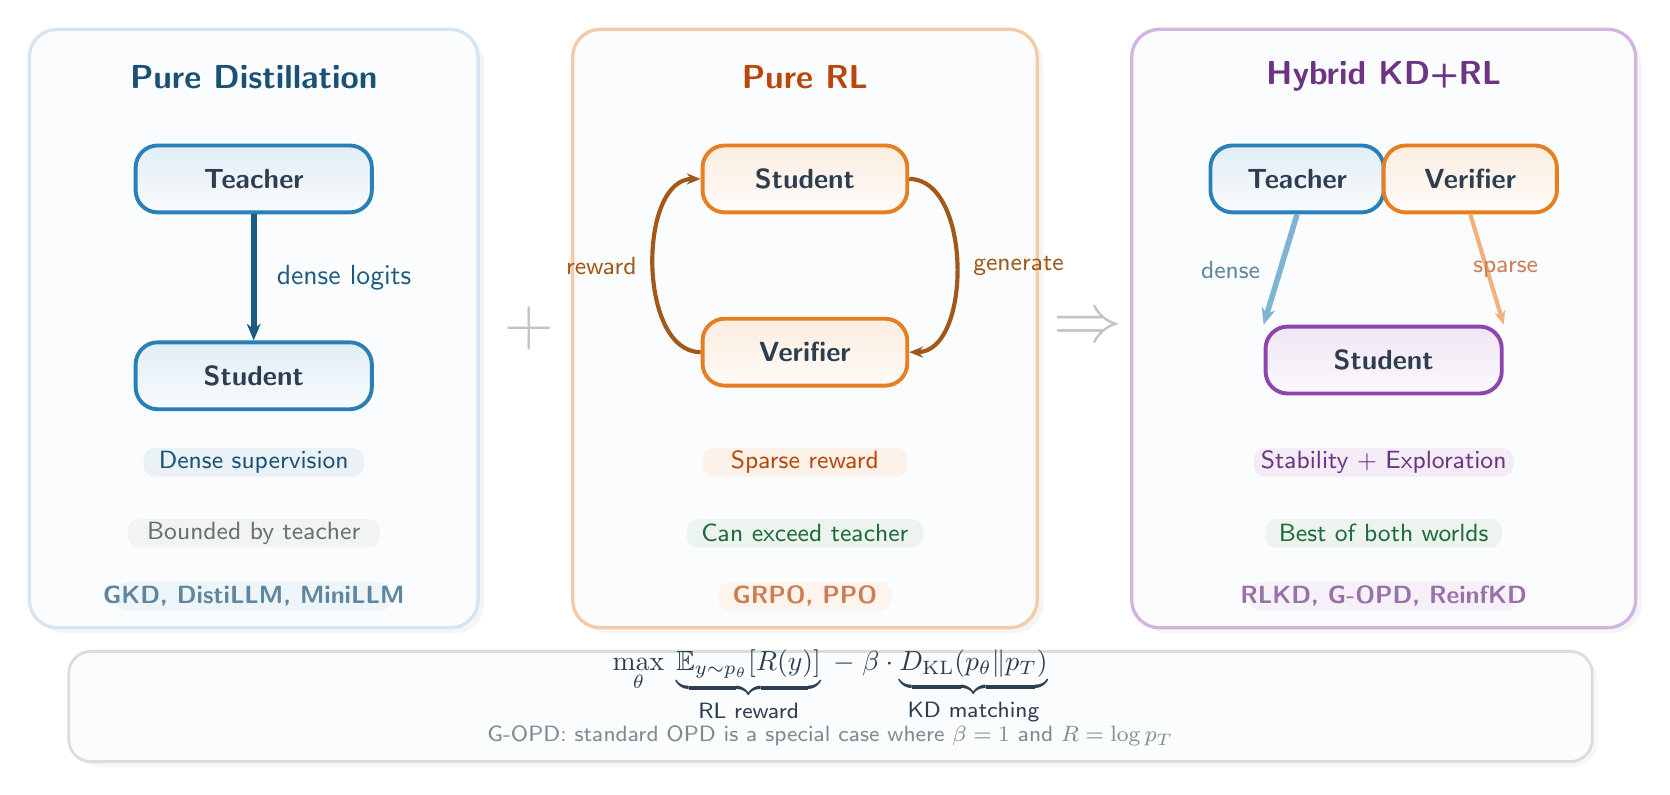
\begin{tikzpicture}[
    >=Stealth,
    mainbox/.style={
      draw=#1, line width=1.4pt, rounded corners=8pt,
      top color=#1!14, bottom color=#1!3,
      font=\normalsize\bfseries, minimum width=2.4cm, minimum height=0.85cm,
      text centered, inner sep=5pt, text=deepgray
    },
    arr/.style={-{Stealth[length=5pt,width=4pt]}, line width=1.5pt, #1},
    thickarr/.style={-{Stealth[length=6pt,width=5pt]}, line width=2pt, #1},
  ]

  % =================== Column 1: Pure Distillation ===================
  % Card
  \fill[black, opacity=0.04, rounded corners=11pt] (0.08, 0.73) rectangle (5.78, 8.33);
  \fill[panelbg, rounded corners=10pt] (0, 0.8) rectangle (5.7, 8.4);
  \draw[lightblue, line width=1.2pt, rounded corners=10pt] (0, 0.8) rectangle (5.7, 8.4);

  \begin{scope}[shift={(2.85, 0)}]
    \node[font=\large\bfseries, deepblue] at (0, 7.8) {Pure Distillation};

    \node[mainbox=midblue, minimum width=3.0cm] (t1) at (0, 6.5) {Teacher};
    \node[mainbox=midblue, minimum width=3.0cm] (s1) at (0, 4.0) {Student};

    \draw[thickarr=midblue!70!black] (t1) -- (s1)
      node[midway, right, font=\normalsize, midblue!70!black, xshift=4pt] {dense logits};

    % Feature pill
    \fill[midblue!10, rounded corners=4pt] (-1.4, 2.72) rectangle (1.4, 3.08);
    \node[font=\small, deepblue] at (0, 2.9) {Dense supervision};

    % Limitation pill
    \fill[midgray!10, rounded corners=4pt] (-1.6, 1.82) rectangle (1.6, 2.18);
    \node[font=\small, midgray!80!black] at (0, 2.0) {Bounded by teacher};

    % Methods pill
    \fill[midblue!8, rounded corners=4pt] (-1.75, 1.02) rectangle (1.75, 1.38);
    \node[font=\small\bfseries, deepblue!70] at (0, 1.2) {GKD, DistiLLM, MiniLLM};
  \end{scope}

  % =================== Plus ===================
  \node[font=\Huge\bfseries, midgray!50] at (6.35, 4.6) {$+$};

  % =================== Column 2: Pure RL ===================
  \fill[black, opacity=0.04, rounded corners=11pt] (6.98, 0.73) rectangle (12.88, 8.33);
  \fill[panelbg, rounded corners=10pt] (6.9, 0.8) rectangle (12.8, 8.4);
  \draw[lightorange, line width=1.2pt, rounded corners=10pt] (6.9, 0.8) rectangle (12.8, 8.4);

  \begin{scope}[shift={(9.85, 0)}]
    \node[font=\large\bfseries, deeporange] at (0, 7.8) {Pure RL};

    \node[mainbox=midorange, minimum width=2.6cm] (s2) at (0, 6.5) {Student};
    \node[mainbox=midorange, minimum width=2.6cm] (v2) at (0, 4.3) {Verifier};

    % Loop — vertical, clean
    \draw[arr=midorange!70!black] (s2.east) .. controls ++(0.8,0) and ++(0.8,0) .. (v2.east)
      node[pos=0.5, right, font=\small, midorange!70!black, xshift=2pt] {generate};
    \draw[arr=midorange!70!black] (v2.west) .. controls ++(-0.8,0) and ++(-0.8,0) .. (s2.west)
      node[pos=0.5, left, font=\small, midorange!70!black, xshift=-2pt] {reward};

    % Feature pill
    \fill[midorange!10, rounded corners=4pt] (-1.3, 2.72) rectangle (1.3, 3.08);
    \node[font=\small, deeporange] at (0, 2.9) {Sparse reward};

    % Advantage pill
    \fill[deepgreen!8, rounded corners=4pt] (-1.5, 1.82) rectangle (1.5, 2.18);
    \node[font=\small, deepgreen] at (0, 2.0) {Can exceed teacher};

    % Methods pill
    \fill[midorange!8, rounded corners=4pt] (-1.1, 1.02) rectangle (1.1, 1.38);
    \node[font=\small\bfseries, deeporange!70] at (0, 1.2) {GRPO, PPO};
  \end{scope}

  % =================== Arrow ===================
  \node[font=\Huge\bfseries, midgray!50] at (13.45, 4.6) {$\Rightarrow$};

  % =================== Column 3: Hybrid KD+RL ===================
  \fill[black, opacity=0.04, rounded corners=11pt] (14.08, 0.73) rectangle (20.48, 8.33);
  \fill[panelbg, rounded corners=10pt] (14.0, 0.8) rectangle (20.4, 8.4);
  \draw[lightpurple, line width=1.2pt, rounded corners=10pt] (14.0, 0.8) rectangle (20.4, 8.4);

  \begin{scope}[shift={(17.2, 0)}]
    \node[font=\large\bfseries, deeppurple] at (0, 7.8) {Hybrid KD+RL};

    \node[mainbox=midblue, minimum width=2.2cm] (t3) at (-1.1, 6.5) {Teacher};
    \node[mainbox=midorange, minimum width=2.2cm] (v3) at (1.1, 6.5) {Verifier};
    \node[mainbox=midpurple, minimum width=3.0cm] (s3) at (0, 4.2) {Student};

    \draw[thickarr=midblue!60] (t3.south) -- (s3.north west)
      node[midway, left, font=\small, deepblue!70, xshift=-3pt] {dense};
    \draw[arr=midorange!60] (v3.south) -- (s3.north east);
    \node[font=\small, deeporange!70] at (1.55, 5.35) {sparse};

    % Feature pill
    \fill[midpurple!10, rounded corners=4pt] (-1.65, 2.72) rectangle (1.65, 3.08);
    \node[font=\small, deeppurple] at (0, 2.9) {Stability + Exploration};

    % Advantage pill
    \fill[deepgreen!8, rounded corners=4pt] (-1.5, 1.82) rectangle (1.5, 2.18);
    \node[font=\small, deepgreen] at (0, 2.0) {Best of both worlds};

    % Methods pill
    \fill[midpurple!8, rounded corners=4pt] (-1.7, 1.02) rectangle (1.7, 1.38);
    \node[font=\small\bfseries, deeppurple!70] at (0, 1.2) {RLKD, G-OPD, ReinfKD};
  \end{scope}

  % =================== Bottom equation box ===================
  \fill[black, opacity=0.03, rounded corners=9pt] (0.58, -0.97) rectangle (19.92, 0.43);
  \fill[panelbg, rounded corners=8pt] (0.5, -0.9) rectangle (19.85, 0.5);
  \draw[midgray!30, line width=1pt, rounded corners=8pt] (0.5, -0.9) rectangle (19.85, 0.5);

  \node[font=\normalsize, deepgray] at (10.17, 0.05) {
    $\displaystyle \max_\theta \;
    \underbrace{\mathbb{E}_{y \sim p_\theta}[R(y)]}_{\text{\footnotesize RL reward}}
    \;-\; \beta \cdot
    \underbrace{D_{\mathrm{KL}}(p_\theta \| p_T)}_{\text{\footnotesize KD matching}}$
  };
  \node[font=\footnotesize, midgray] at (10.17, -0.58) {
    G-OPD: standard OPD is a special case where $\beta = 1$ and $R = \log p_T$
  };

\end{tikzpicture}
\end{document}
